\documentclass[12pt]{article}
\usepackage{inputenc}
\usepackage[top=1in, bottom=1in, left=1in, right=1in]{geometry}
\usepackage{setspace}
\usepackage{parskip}
\setcounter{secnumdepth}{1}
\pagestyle{plain}
\usepackage{graphicx}
%\usepackage{fontspec}
%\setmainfont{Georgia}
\setlength{\parindent}{0 cm}
\usepackage[section]{placeins}


\usepackage[compact]{titlesec}  
\usepackage{amssymb}
\usepackage{amsmath}
\newcommand\numberthis{\addtocounter{equation}{1}\tag{\theequation}}
\titlespacing{\section}{0pt}{0pt}{0pt}
\usepackage{changepage}
\newenvironment{myenv}{\begin{adjustwidth}{1cm}{}}{\end{adjustwidth}}

\begin{document}
% Manual Heading
{\raggedleft{}Gabriel Griggs} \\
Professor Mark Alber \\
Nonlinear Dynamical Systems: ACMS 403630-01 \\
Tuesday, February 11 2014\\
Homework 2
\section*{Question 1}
\begin{myenv}
\textbf{Question:} Use a calculator to iterate each of the following functions (using an arbitrary initial value) and explain these results.

\textbf{Answer:} Using a MATLAB script, we are able to make tables of values for the various functions over various iterations: \\

a) $C(x) = cos(x)$ : from points below, it appears that this function is converging to a spiraling fixed point located roughly at .735. Using a cobweb diagram, this appears to be confirmed.


\begin{table}[h]
\begin{tabular}{llllll}
iteration from x0 = & -1    & -0.5  & 0     & 0.5   & 1     \\
1                   & 0.540 & 0.878 & 1.000 & 0.878 & 0.540 \\
2                   & 0.858 & 0.639 & 0.540 & 0.639 & 0.858 \\
3                   & 0.654 & 0.803 & 0.858 & 0.803 & 0.654 \\
4                   & 0.793 & 0.695 & 0.654 & 0.695 & 0.793 \\
5                   & 0.701 & 0.768 & 0.793 & 0.768 & 0.701 \\
6                   & 0.764 & 0.719 & 0.701 & 0.719 & 0.764 \\
7                   & 0.722 & 0.752 & 0.764 & 0.752 & 0.722 \\
8                   & 0.750 & 0.730 & 0.722 & 0.730 & 0.750 \\
9                   & 0.731 & 0.745 & 0.750 & 0.745 & 0.731 \\
10                  & 0.744 & 0.735 & 0.731 & 0.735 & 0.744
\end{tabular}
\end{table}

\begin{figure} [H]
    \centering
    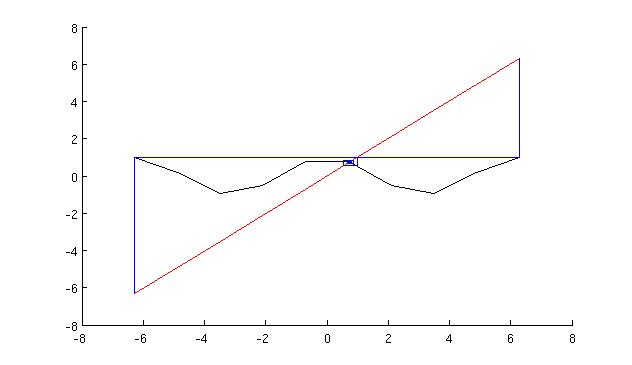
\includegraphics[width=0.8\textwidth]{cobweb1a}
    \caption{Cobweb: 1a}
    \label{figure:a0}
\end{figure}

b) $S(x) = sin(x)$ : in the window from $[-1,1]$ it is not clear what exactly the behavior of this function is. From the cobweb graph, however, it appears to be converging very slowly to a sink at the origin.

\begin{table}[h]
\begin{tabular}{llllll}
iteration from x0 = & -1     & -0.5   & 0     & 0.5   & 1     \\
1                   & -0.841 & -0.479 & 0.000 & 0.479 & 0.841 \\
2                   & -0.746 & -0.461 & 0.000 & 0.461 & 0.746 \\
3                   & -0.678 & -0.445 & 0.000 & 0.445 & 0.678 \\
4                   & -0.628 & -0.431 & 0.000 & 0.431 & 0.628 \\
5                   & -0.587 & -0.417 & 0.000 & 0.417 & 0.587 \\
6                   & -0.554 & -0.405 & 0.000 & 0.405 & 0.554 \\
7                   & -0.526 & -0.394 & 0.000 & 0.394 & 0.526 \\
8                   & -0.502 & -0.384 & 0.000 & 0.384 & 0.502 \\
9                   & -0.481 & -0.375 & 0.000 & 0.375 & 0.481 \\
10                  & -0.463 & -0.366 & 0.000 & 0.366 & 0.463
\end{tabular}
\end{table}

\begin{figure} [H]
    \centering
    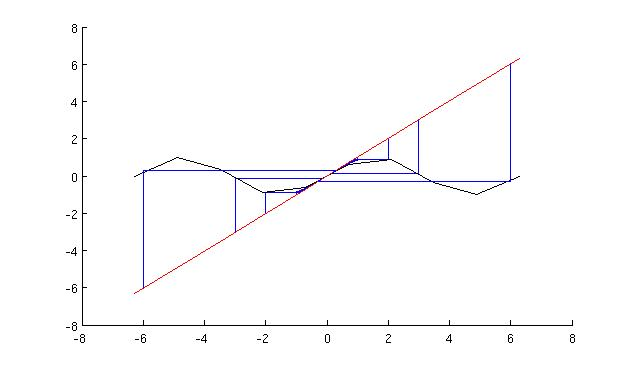
\includegraphics[width=0.8\textwidth]{cobweb1b}
    \caption{Cobweb: 1b}
    \label{figure:a1}
\end{figure}

c) $E(x) = exp(x)$ : from the table below, as well as the cobweb graph, it would appear that there are no fixed points for this function and that all points go to infinity.

\begin{table}[h]
\begin{tabular}{llllll}
iteration from x0 = & -1       & -0.5      & 0        & 0.5      & 1        \\
1                   & 3.68E-01 & 6.07E-01  & 1.00E+00 & 1.65E+00 & 2.72E+00 \\
2                   & 1.44E+00 & 1.83E+00  & 2.72E+00 & 5.20E+00 & 1.52E+01 \\
3                   & 4.24E+00 & 6.26E+00  & 1.52E+01 & 1.81E+02 & 3.81E+06 \\
4                   & 6.94E+01 & 5.23E+02  & 3.81E+06 & 5.64E+78 & Inf      \\
5                   & 1.43E+30 & 1.14E+227 & Inf      & Inf      & Inf      \\
6                   & Inf      & Inf       & Inf      & Inf      & Inf      \\
7                   & Inf      & Inf       & Inf      & Inf      & Inf      \\
8                   & Inf      & Inf       & Inf      & Inf      & Inf      \\
9                   & Inf      & Inf       & Inf      & Inf      & Inf      \\
10                  & Inf      & Inf       & Inf      & Inf      & Inf     
\end{tabular}
\end{table}

\begin{figure} [H]
    \centering
    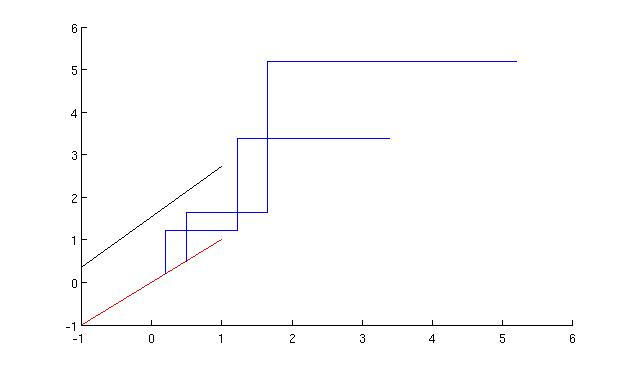
\includegraphics[width=0.8\textwidth]{cobweb1c}
    \caption{Cobweb: 1c}
    \label{figure:a2}
\end{figure}

d) $F(x) = \frac{1}{e}e^x$ : this function appears to be converging to a fixed point at (1,1), confirmed both by the table below and the cobweb graph.

\begin{table}[h]
\begin{tabular}{llllll}
iteration from x0 = & -1    & -0.5  & 0     & 0.5   & 1     \\
1                   & 0.135 & 0.223 & 0.368 & 0.607 & 1.000 \\
2                   & 0.421 & 0.460 & 0.531 & 0.675 & 1.000 \\
3                   & 0.561 & 0.583 & 0.626 & 0.722 & 1.000 \\
4                   & 0.644 & 0.659 & 0.688 & 0.758 & 1.000 \\
5                   & 0.701 & 0.711 & 0.732 & 0.785 & 1.000 \\
6                   & 0.741 & 0.749 & 0.765 & 0.806 & 1.000 \\
7                   & 0.772 & 0.778 & 0.790 & 0.824 & 1.000 \\
8                   & 0.796 & 0.801 & 0.811 & 0.839 & 1.000 \\
9                   & 0.816 & 0.819 & 0.828 & 0.851 & 1.000 \\
10                  & 0.832 & 0.835 & 0.842 & 0.861 & 1.000
\end{tabular}
\end{table}

\begin{figure} [H]
    \centering
    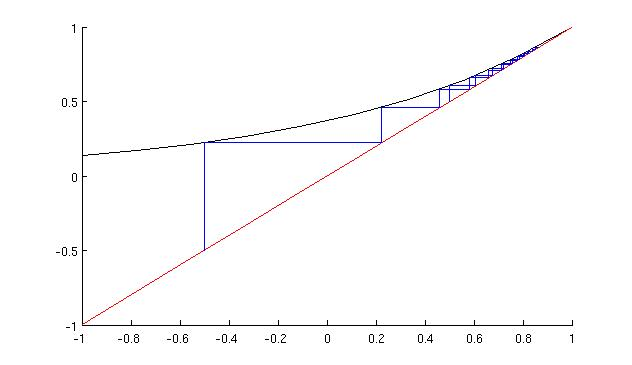
\includegraphics[width=0.8\textwidth]{cobweb1d}
    \caption{Cobweb: 1d}
    \label{figure:a3}
\end{figure}

e) $A(x) = arctan(x)$ : this function appears to be converging to a fixed point at the origin, which is confirmed by the fact that 0 returns nothing but itself and by the cobweb graph.

\begin{table}[h]
\begin{tabular}{llllll}
iteration from x0 = & -1     & -0.5   & 0     & 0.5   & 1     \\
1                   & -0.785 & -0.464 & 0.000 & 0.464 & 0.785 \\
2                   & -0.666 & -0.434 & 0.000 & 0.434 & 0.666 \\
3                   & -0.587 & -0.410 & 0.000 & 0.410 & 0.587 \\
4                   & -0.531 & -0.389 & 0.000 & 0.389 & 0.531 \\
5                   & -0.488 & -0.371 & 0.000 & 0.371 & 0.488 \\
6                   & -0.454 & -0.355 & 0.000 & 0.355 & 0.454 \\
7                   & -0.426 & -0.341 & 0.000 & 0.341 & 0.426 \\
8                   & -0.403 & -0.329 & 0.000 & 0.329 & 0.403 \\
9                   & -0.383 & -0.318 & 0.000 & 0.318 & 0.383 \\
10                  & -0.366 & -0.308 & 0.000 & 0.308 & 0.366
\end{tabular}
\end{table}

\begin{figure} [H]
    \centering
    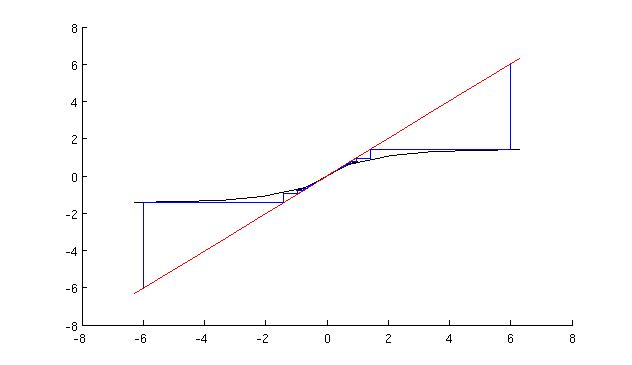
\includegraphics[width=0.8\textwidth]{cobweb1e}
    \caption{Cobweb: 1e}
    \label{figure:a4}
\end{figure}

\end{myenv}

\section*{Question 2}
\begin{myenv}
\textbf{Question:} Using the graph of the function, identify the fixed points for each of the maps in Problem 1:

\textbf{Answer:} 

a) $C(x) = cos(x)$ : Using the graph, as well as the secant method (set to solve for x - f(x) = 0), we can confirm that there is a fixed point at the location $ x = .73908$.

\begin{figure} [H]
    \centering
    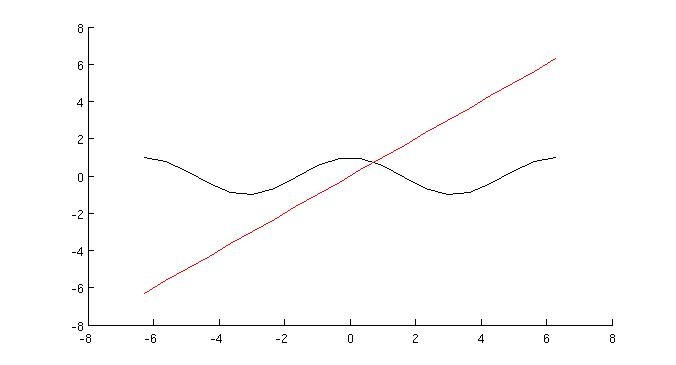
\includegraphics[width=0.8\textwidth]{secant2a}
    \caption{Intersection with y = x for 2a at x = .73908}
    \label{figure:a4}
\end{figure}

b) $S(x) = sin(x)$ : Using the graph, as well as the secant method (set to solve for x - f(x) = 0), we can confirm that there is a fixed point at the location $ x = 0$.

\begin{figure} [H]
    \centering
    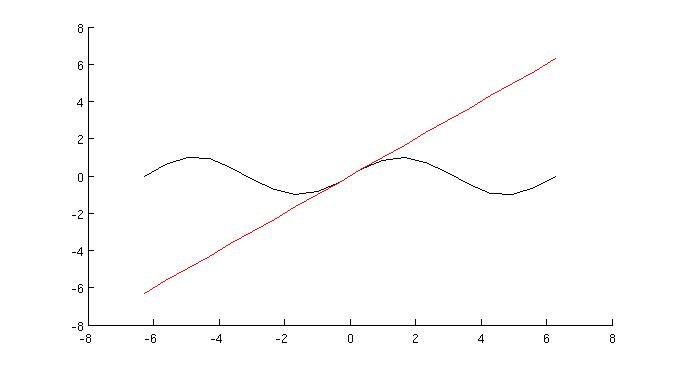
\includegraphics[width=0.8\textwidth]{secant2b}
    \caption{Intersection with y = x for 2b at x = 0}
    \label{figure:a4}
\end{figure}

c) $E(x) = exp(x)$ : Using the graph, as well as the secant method (set to solve for x - f(x) = 0), we can confirm that there is no fixed point for this function as there is no intersection between $C(x) and y = x$.

\begin{figure} [H]
    \centering
    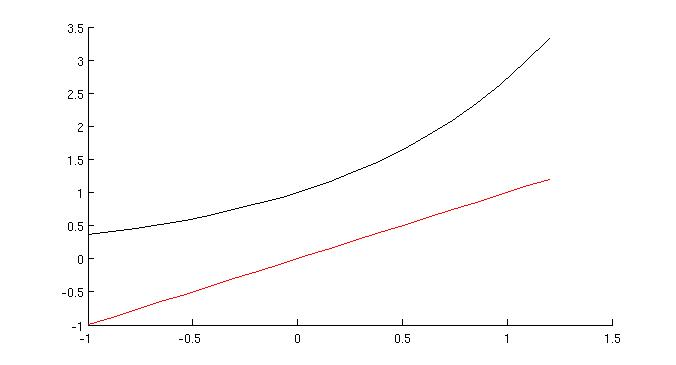
\includegraphics[width=0.8\textwidth]{secant2c}
    \caption{No intersection and, therefore, no fixed point.}
    \label{figure:a4}
\end{figure}

d) $F(x) = \frac{1}{e}exp(x)$ : Using the graph, as well as the secant method (set to solve for x - f(x) = 0), we can actually see that there is not intersection (though $y=x$ gets awfully close to touching $F(x)$). The cobweb is interesting in that it reveals something close to a fixed point, spiral sink.

\begin{figure} [H]
    \centering
    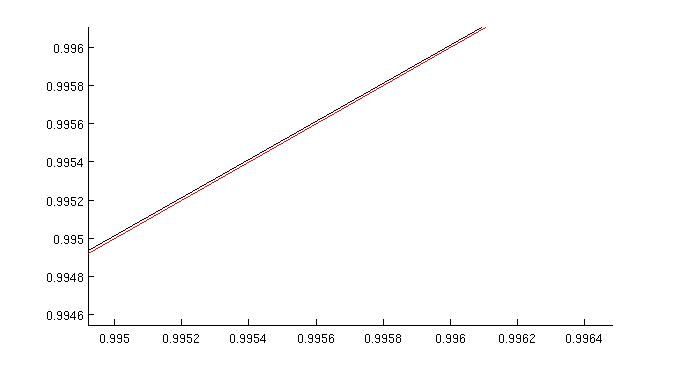
\includegraphics[width=0.8\textwidth]{secant2d}
    \caption{This graph, and secant method analysis, reveals an \emph{almost intersection} point very close to $x=1$. }
    \label{figure:a4}
\end{figure}

e) $A(x) = arctan(x)$ : Using the graph, as well as the secant method (set to solve for x - f(x) = 0), we can see that there is an intersection at the origin. The secant method actually fails to achieve $10^-3$ tolerance within 100 iterations. However, $arctan(0) = 0$ is confirmed explicitly.

\begin{figure} [H]
    \centering
    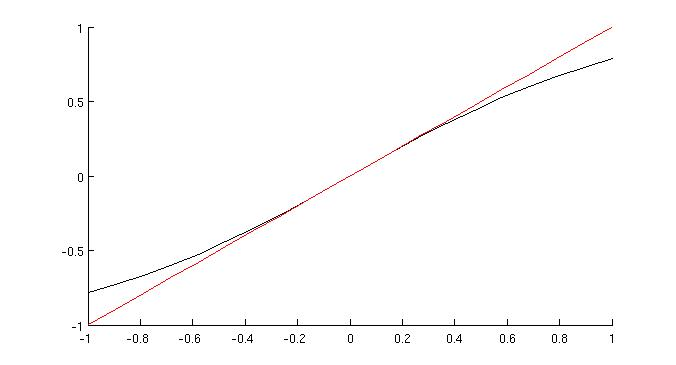
\includegraphics[width=0.8\textwidth]{secant2e}
    \caption{This graph reveals a fixed point at the origin. }
    \label{figure:a4}
\end{figure}

\end{myenv}

\section*{Question 3}
\begin{myenv}
\textbf{Question:} List all periodic points for each of the following maps. Then use the graph of $f(x)$ to sketch the phase portrait for $f(x)$ on the listed intervals.

\textbf{Answer:} 

a) $f(x) = (-0.5)x$ on the interval $(-\infty < x < \infty)$ has the periodic point (and fixed point) $x = 0$. The fact that this is the only periodic point can be seen by the first ten iterations of $f(x)$ which yield: \\

 $- 0.5\, x,\; 0.25\, x,\; - 0.125\, x,\; 0.0625\, x,\;- 0.03125\, x,\; 0.015625\, x,\; - 0.0078125\, x,\;$
 
 $0.00390625\, x,\; - 0.001953125\, x,\; 0.0009765625\, x$.
 
 All of these points have only the periodic point at 0. This can be further verified by setting $f^k(x) - x = 0$ and solving for $x$. In all of these iterations, the only solution is $x = 0$.

\begin{figure} [H]
    \centering
    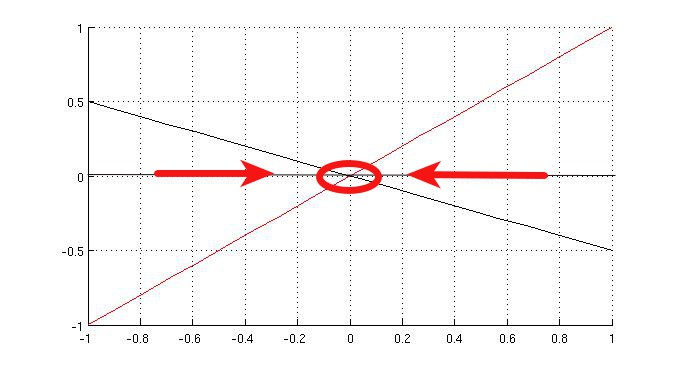
\includegraphics[width=0.8\textwidth]{2_3a}
    \caption{This graph reveals a fixed point at the origin. Note: no matter how far this graph is extended on the axes, it will always look the same as it has its only fixed point at the origin. In other words, on the interval $(-\infty < x < \infty)$, it will look exactly the same as this graph. }
    \label{figure:a4}
\end{figure}

b) $f(x) = -3x$ on the interval $(-\infty < x < \infty)$ has only the periodic (and fixed) point at the origin. Again, this can be verified by looking at the first ten iterations of the function:

$- 3\, x,\; 9\, x,\; - 27\, x,\; 81\, x,\; - 243\, x,\; 729\, x,\; - 2187\, x,\; 6561\, x,\; - 19683\, x,\; 59049\, x$

 All of these points have only the periodic point at 0. This can be further verified by setting $f^k(x) - x = 0$ and solving for $x$. In all of these iterations, the only solution is $x = 0$.
 
\begin{figure} [H]
    \centering
    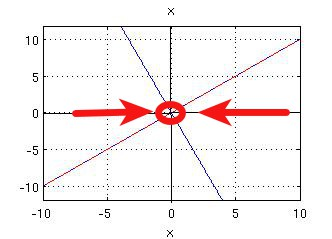
\includegraphics[width=0.8\textwidth]{2_3b}
    \caption{This graph reveals a fixed point at the origin. Note: no matter how far this graph is extended on the axes, it will always look the same as it has its only fixed point at the origin. In other words, on the interval $(-\infty < x < \infty)$, it will look exactly the same as this graph. }
    \label{figure:a4}
\end{figure}

c) $f(x) = x-x^2$ on the interval $[0 \le x \le 1]$ has periodic points at the fixed point $x = 0$. This can be further verified by analysis of various iterations, shown below:

$x - x^2,\; x - {\left(x - x^2\right)}^2 - x^2,\; x - {\left(x - x^2\right)}^2 - x^2 - {\left({\left(x - x^2\right)}^2 - x + x^2\right)}^2$

In setting all of these equations equal to $x$ and solving for the zero, using the secant method, and verifying with the graphs, we can see that the only $x = 0$ returns itself. See the graphs below:

\begin{figure} [H]
    \centering
    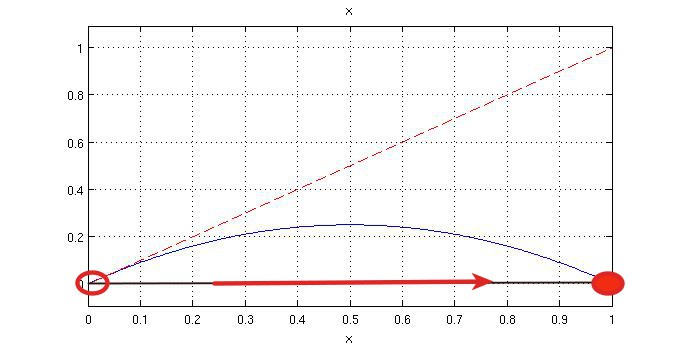
\includegraphics[width=0.8\textwidth]{2_3c}
    \caption{This graph reveals a fixed point at the origin (unstable) and at $x = 1$ (stable).}
    \label{figure:a4}
\end{figure}

\begin{figure} [H]
    \centering
    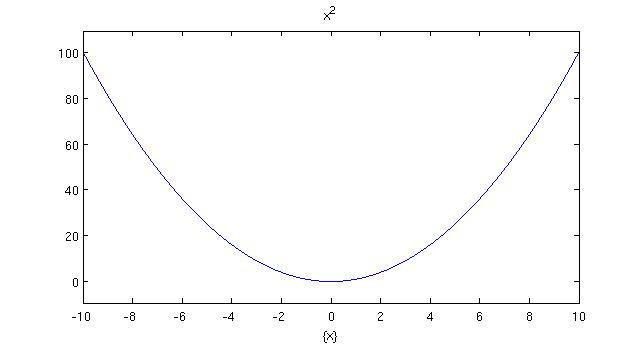
\includegraphics[width=0.8\textwidth]{2_3c_1}
    \caption{This graph reveals the only periodic point at $x=0$ for the first iteration of the function minus x, which is confirmed by the secant method.}
    \label{figure:a4}
\end{figure}

\begin{figure} [H]
    \centering
    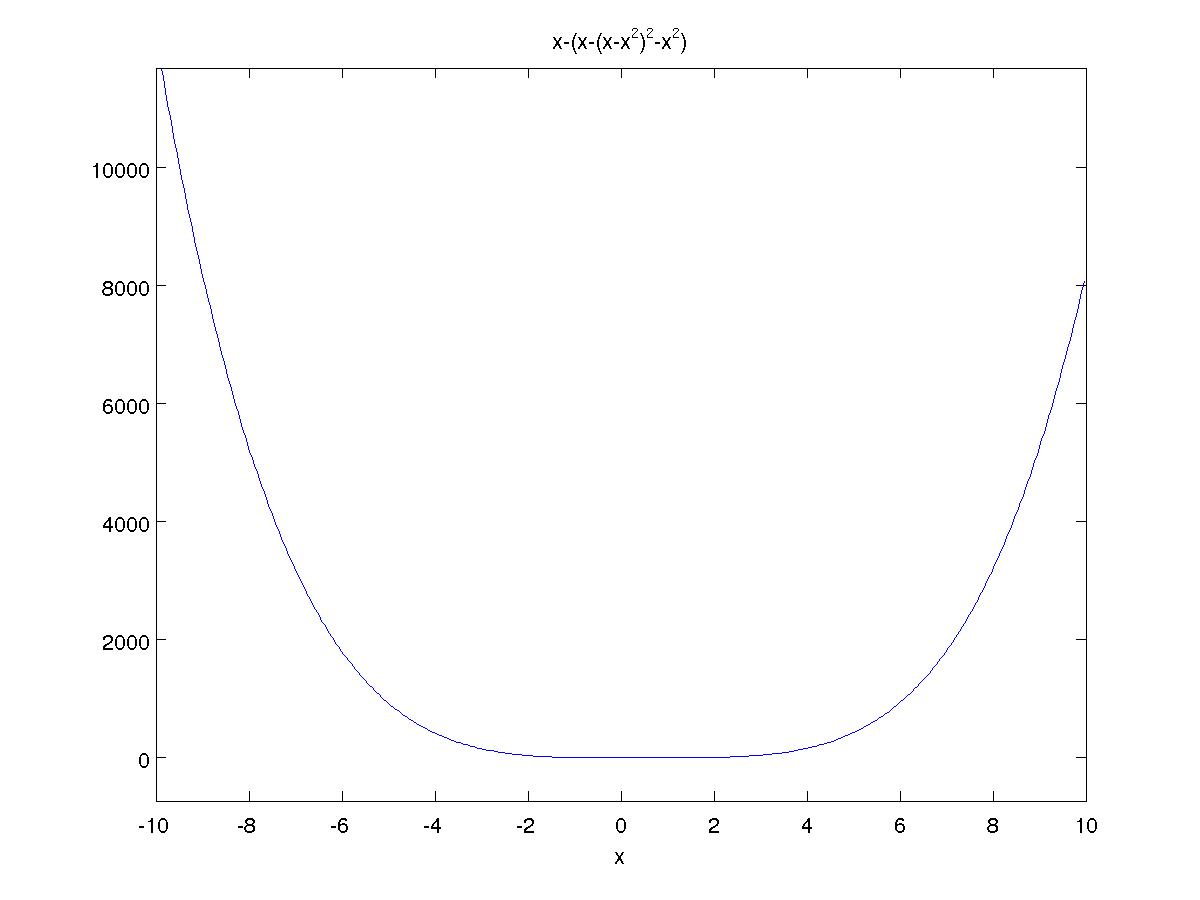
\includegraphics[width=0.8\textwidth]{2_3c_2}
    \caption{This graph reveals the only periodic point at $x=0$ for the second iteration of the function minus x, which is confirmed by the secant method.}
    \label{figure:a4}
\end{figure}

\begin{figure} [H]
    \centering
    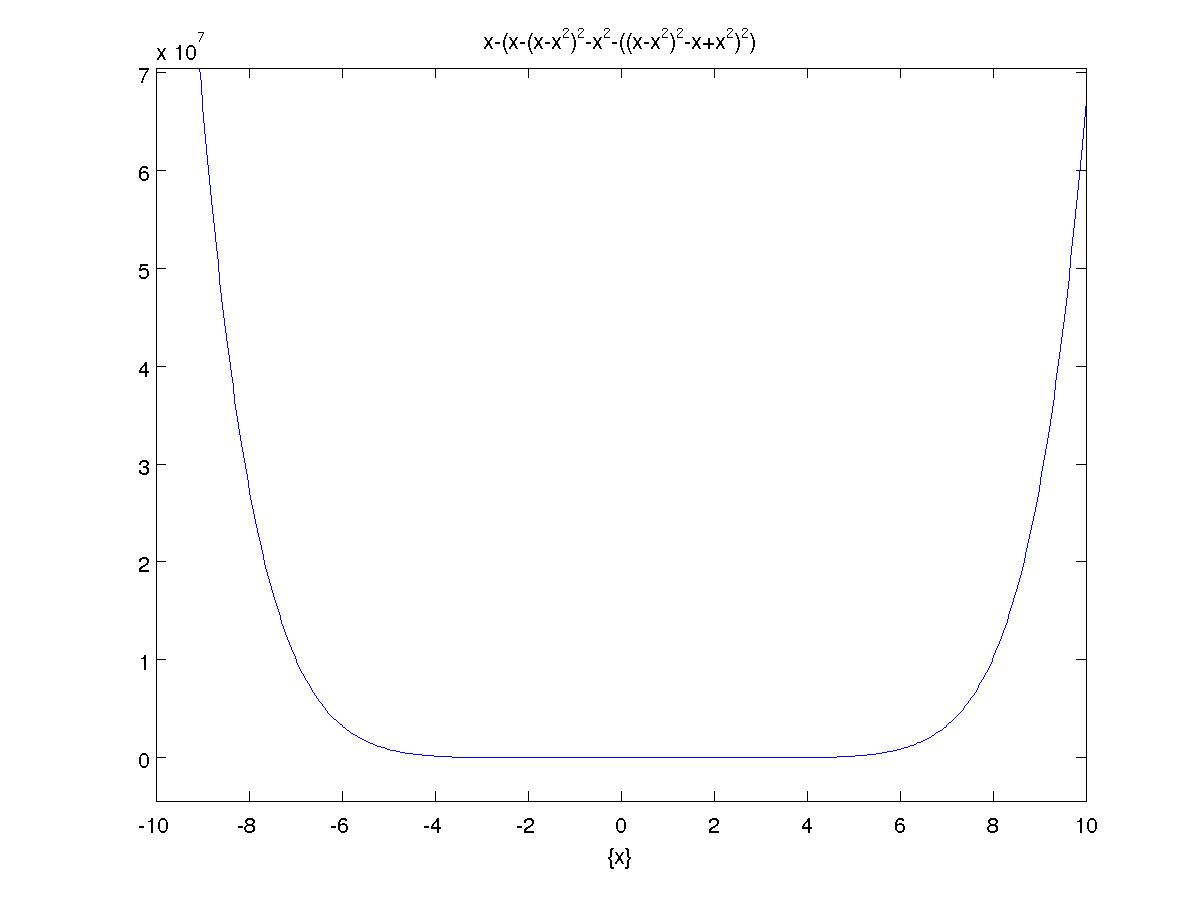
\includegraphics[width=0.8\textwidth]{2_3c_3}
    \caption{This graph reveals the only periodic point at $x=0$ for the third iteration of the function minus x, which is confirmed by the secant method.}
    \label{figure:a4}
\end{figure}
\end{myenv}

\section*{Question 4}
\begin{myenv}
\textbf{Question:} Identify the stable sets of each of the fixed points for the maps in Problem 3.

\textbf{Answer:}

a) $f(x) = -(0.5)x$ --- the stable set of this function's fixed point, at the origin, consists of all points in the interval $(-\infty, \infty)$ because the sequence $f^k(x)$, where $x \in (-\infty,\infty)$, converges to 0. In other words, $W^s(0) = (-\infty,\infty)$.

b) $f(x) = -(3)x$ --- the stable set of this function's fixed point, at the origin, consists of all points in the interval $(-\infty, \infty)$ because the sequence $f^k(x)$, where $x \in (-\infty,\infty)$, converges to 0. In other words, $W^s(0) = (-\infty,\infty)$.

c) $f(x) = x-x^2$ --- interestingly, it appears that the stable set of the fixed point at $x=1$ consists only the point $x=1$ as it appears that the sequence $f^k(x)$ is forward asymptotic to $0$ on the interval $[0,\infty)$. This makes sense in looking at the kth-iterations in that it is going to be dominated by the negative terms such as $-x^2$ and $-((x-x^2)^2-x+x^2)^2$ --- at a much higher rate for values of $x$ greater than $1$, but still asymptotically for values smaller than $1$ as well.

\end{myenv}

\section*{Question 5}
\begin{myenv}
\textbf{Question:} For each of the following functions, list all critical points and decide whether each is degenerate or non-degenerate.

\textbf{Answer:} According to the definition given in class, a point is critical if $F'(x) = 0$. The critical point is non-degenerate if $F''(x)\neq0$ and degenerate if $F''(x) = 0$.

a) $F(x) = x^3 - x$ has non-degenerate critical points at $x = \pm\sqrt(1/3)$.
	\begin{alignat*}{3}
	F'(x) &= 3x^2 - 1 \\
	3x^2 - 1 &= 0 \text{ at } x = \pm\sqrt(1/3) \\
	F''(x) &= 6x \text{ which is $\neq0$ at } x &= \pm\sqrt(1/3)
	\end{alignat*}
	
b) $S(x) = sin(x)$ has non-degenerate critical points at $ \frac{(2n+1)\pi}{2}$ for $n = 0,1,2,...$.
	\begin{alignat*}{3}
	S'(x) &= cos(x) \\
	cos(x) &= 0 \text{ at } \frac{(2n+1)\pi}{2} \text{ for } n = 0,1,2,...\\
	S''(x) &= -sin(x) \text{ which is $\neq0$ at } x = \frac{(2n+1)\pi}{2} \text{ for } n = 0,1,2,...
	\end{alignat*}
	
c) $f(x) = x^4-2x^2$ has non-degenerate critical points at $x = 0, \pm1$.
	\begin{alignat*}{3}
	f'(x) &= 4x^3 - 4x \\
	x(4x^2-4) &= 0 \text{ at } x = 0, \pm1\\
	f''(x) &= 12x-4 \text{ which is $\neq0$ at } x = 0, \pm1
	\end{alignat*}

d) $g(x) = x^3 + x^4$ has a degenerate critical point at $x = 0$ and a non-degenerate point at $x = \frac{-3}{4}$.
	\begin{alignat*}{3}
	g'(x) &= 3x^2 + 4x^3 \\
	x^2(3+4x) &= 0 \text{ at } x = 0, \frac{-3}{4}\\
	g''(x) &= 6x + 12x^2 \text{ which is $\neq0$ at } x = \frac{-3}{4} \text{ and which is $=0$ at } x = 0.
	\end{alignat*}

\end{myenv}


\end{document}

